Após o carregamento e união dos \textit{datasets}, explorei os dados através de nodos estatísticos.

\begin{figure}[H]
    \centering
    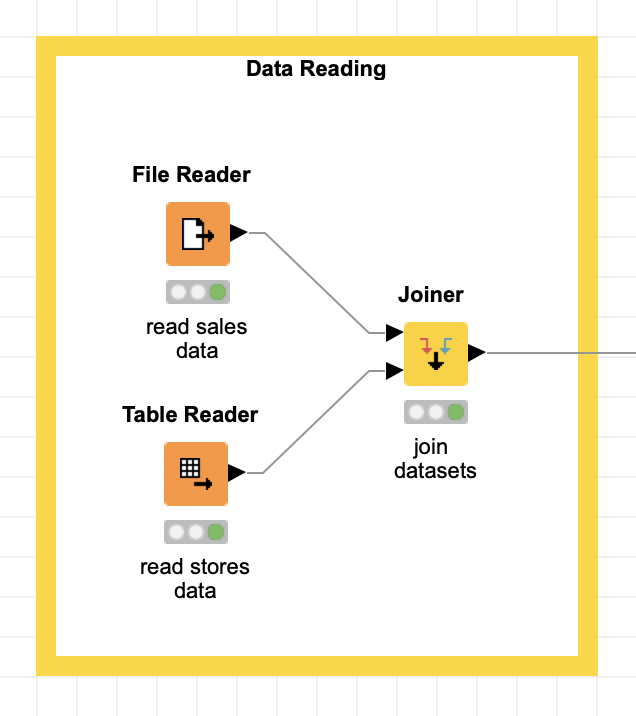
\includegraphics[scale=0.5]{Images/T1_a.png}
    \caption{Carregamento e união dos datasets}
\end{figure}

\begin{figure}[H]
    \centering
    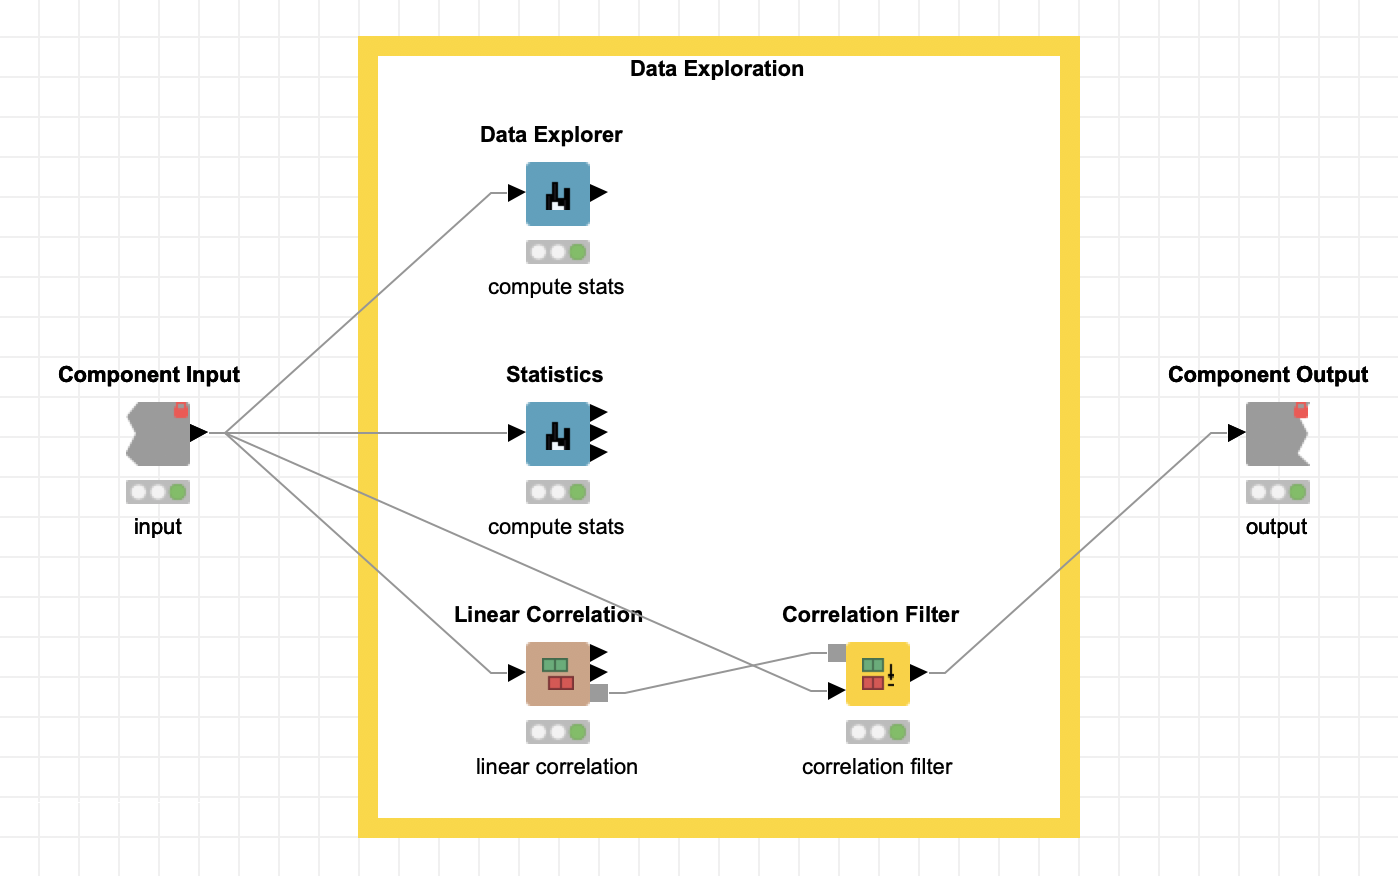
\includegraphics[scale=0.4]{Images/T1_b.png}
    \caption{Exploração dos dados}
\end{figure}

\clearpage

O \textit{workflow} foi desenvolvido dentro de um \textit{component} de modo a poder obter todas as \textit{views} numa só página.

\begin{figure}[H]
    \centering
    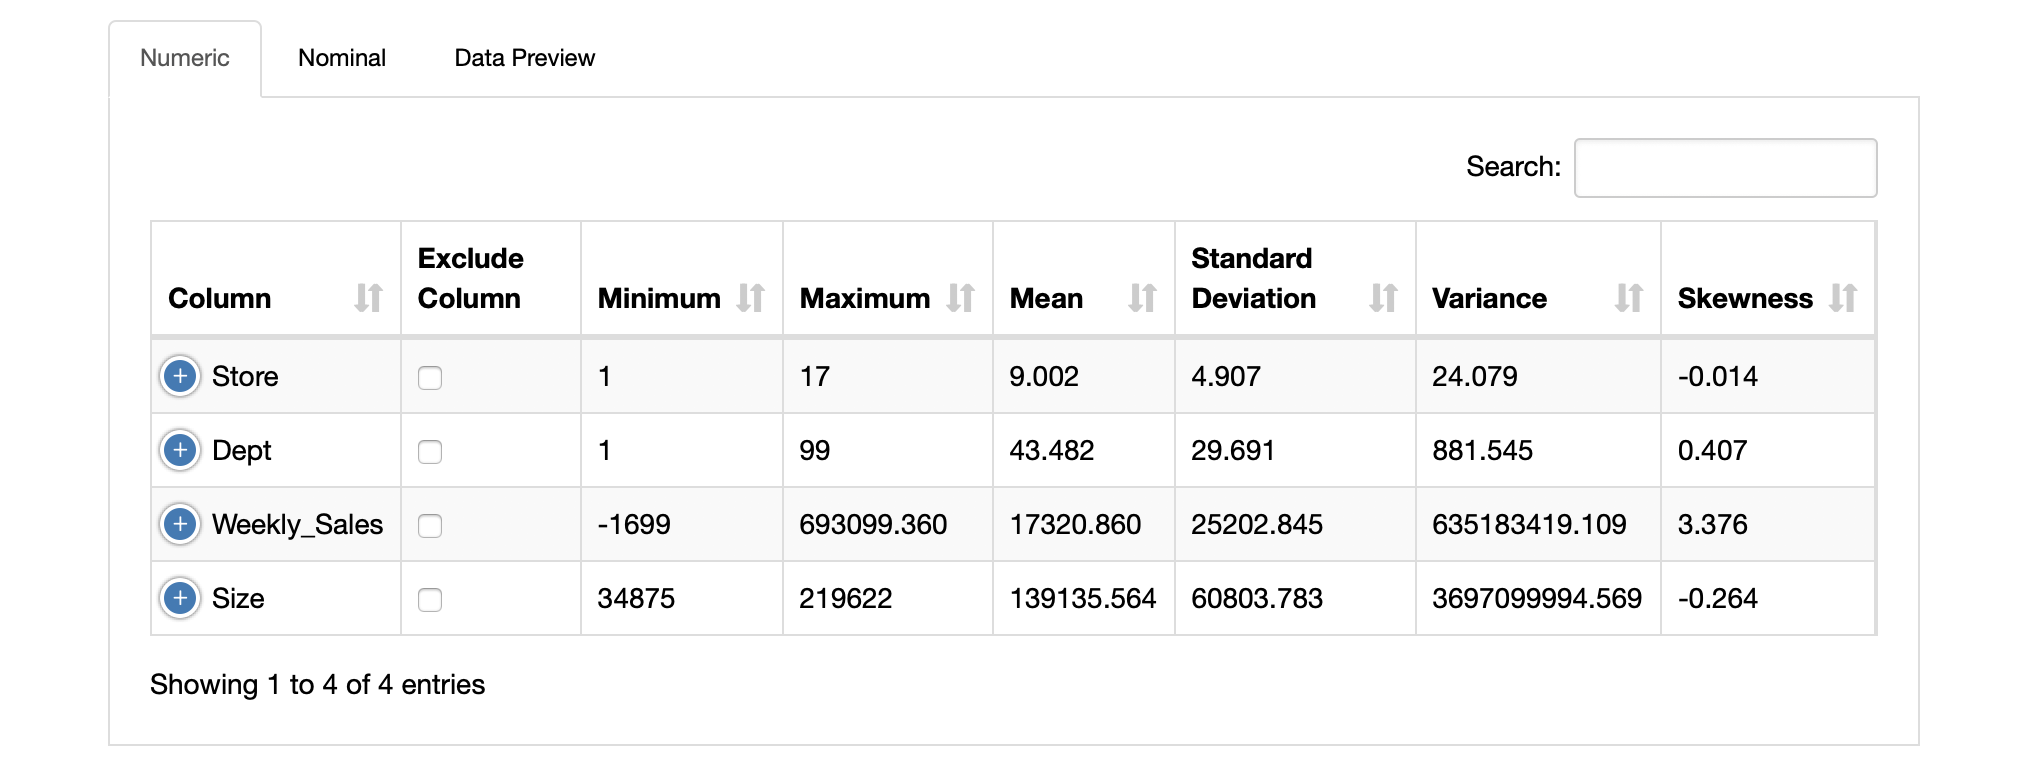
\includegraphics[scale=0.3]{Images/T1_c.png}
    \caption{Vista gráfica interativa}
\end{figure}